% \documentclass{book}
% \usepackage[utf8]{inputenc}
% \usepackage{graphicx}
% \graphicspath{{files/}}
% \usepackage{amssymb}
% \usepackage{amsmath,amsfonts,amssymb,amsthm}
% \usepackage{mathtools}
% \usepackage{subfiles}
% \usepackage{biblatex}
% \newcommand{\horrule}[1]{\rule{\linewidth}{#1}}% Create horizontal rule command with 1 argument of height
% \let\oldnorm\norm   % <-- Store original \norm as \oldnorm
% \let\norm\undefined % <-- "Undefine" \norm
% \DeclarePairedDelimiter\norm{\lVert}{\rVert}
% \newtheorem{definition}{Definition}
% \newtheorem{theorem}{Theorem}

% contributors: 0/Nihaar Shah, 2/Cynthia Gao, 1/Alper Cakan

% \begin{document}



\chapter{Test}
\begin{refsection}
  % contributors: Nihaar Shah
\section{Poincar\'e Embeddings for Hierarchical Representations}
We start by discussing \cite{Poincar\'e}. In this paper, the authors introduce a new approach for learning hierarchical representations of symbolic data by embedding them into hyperbolic space and more specifically into an n-dimensional Poincare ball. The motivation for this is to capture latent hierarchical structure in complex symbolic datasets which is often lost by merely embedding into a Euclidean vector space. The efficient algorithm introduced here to learn the embeddings empirically shows superior performance than Euclidean ones both in terms of the representation capacity as well as generalization ability. 
\\ Generally, similarity between objects in the embedding space is measured primarily in terms of their distance and/or inner product (hence their orientation). Here we consider the distances as a measure. 
\subsection{Preliminaries}
\subsubsection{Hyperbolic space}
Hyperbolic space is a space exhibiting Hyperbolic geometry. The primary difference from Euclidean geometry is that the parallel axiom of Euclidean geometry (i.e. parallel lines do not intersect) doesn't hold in Hyperbolic geometry while the remaining axioms do hold.
\begin{figure}
    \centering
    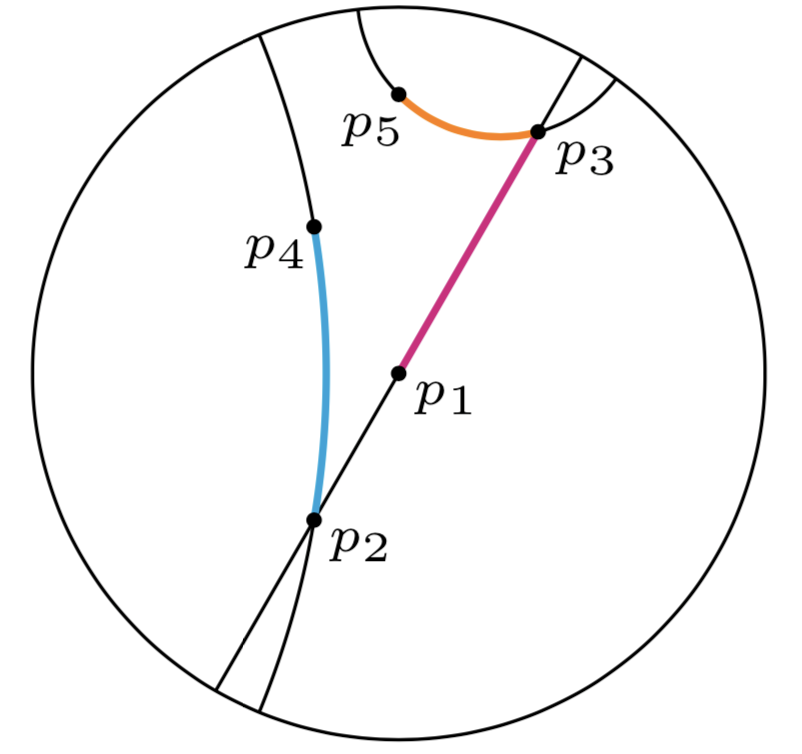
\includegraphics[width=.4\textwidth]{chapter_14/files/poincare1.png}
    \caption{Geodesics of a Poincare disk. Note the hyperbolic disk area and the circle length grow exponentially the closer they are to the boundary. }
    \label{hyperb-tree}
\end{figure}
Informally, hyperbolic space can be thought of as a continuous version of trees and a space with constant negative curvature. This relationship between hyperbolic space and a tree can be visualised by considering the growth rate of branches (b) of a tree as the level (l) of the tree progresses. For a branching factor b a tree has $$(b+1)b^{l-1}$$ nodes at level 'l' while $$((b+1)b^l-2)/(b-1)$$ nodes on a level $\leq l$. The number of children grows exponentially with distance from the root. In hyperbolic geometry, this relation can be modeled naturally because the disc area and circle length grow exponentially with radius (as compared to the Euclidean distance). Consider the 2 dimensional hyperbolic space with constant curvature $K=-1$ where the length of a circle is $$2 \pi \text{sinh} r = 2 \pi ((e^r - e^{-r})-1)$$ and the disc area is $$2 \pi (cosh r -1) =2 \pi ((e^r + e^{-r})-1)$$. Thus both disc area and the circle length grow exponentially with r (relative to their euclidean distance) as also illustrated in fig \ref{hyperb-tree}.
\subsubsection{Poincare Embeddings}
Particularly, the model of hyperbolic space being considered is a Poincare ball model because it lends itself to gradient based Riemann optimization ( shall be discussed) which is easily parallelizable.
\\This paper wishes to reflect the latent hierarchy in which symbols can be organized in the embedding space in two ways:
\begin{itemize}
    \item Inducing an appropriate bias on the structure 
    \item Capturing the hierarchy explicitly in the embedding space to gain insights about the relationships between symbols and the importance of individual symbols.
\end{itemize}
Crucially, the information about hierarchy e.g. ordered input pairs is not directly accessible and hence the task of inferring these relationships in a fully unsupervised way is tackled by embedding the symbolic data into Hyperbolic space $\mathbb{H}$.
\bigskip
\\Let us define an open d-dimensional unit ball where $\norm{.}$ is th Euclidean norm 
$$\mathbb{B}^d = \{\mathbf{x} \in R^d | \norm{\mathbf{x}}<1\}$$
The Poincare ball model of hyperbolic space corresponds then to the Riemannian manifold $(\mathbb{B}^d,g_x)$ which is the open unit ball with Riemannian metric tensor\footnote[1]{A metric tensor is a type of function which takes as input a pair of tangent vectors v and w at a point of a surface and produces a real number scalar g(v, w).  A manifold equipped with a positive-definite $(g(v, v) > 0$ to every nonzero vector v) metric tensor is known as a Riemannian manifold.}:
$$g_x = (\frac{2}{1 - \norm{\mathbf{x}}^2})^2 g^E$$
Here $\mathbf{x} \in B^d$ and $g^E$ denotes the Euclidean metric tensor. The distance between points $\mathbf{u,v}\in \mathbb{B}^d$ is:
\begin{equation}
    d(\mathbf{u,v}) = \text{arcosh }(1+ \frac{2 \norm{\mathbf{u - v}}^2}{(1 - \norm{\mathbf{u}}^2)(1 - \norm{\mathbf{v}}^2)})\label{dist-poin}
\end{equation}
The above equation \ref{dist-poin} crucially shows that the distance within the Poincare ball changes smoothly with respect to location $\mathbf{u}$ and $\mathbf{v}$ - a locality property which will be key to finding continuous embeddings of hierarchies.
\subsection{Optimization}
Let:
$$\mathbb{T}_\theta \mathbb{B} \text{ - denote the tangent space of a point} \mathbf{\theta} \in B^d$$ 

$$\nabla_R \in \mathbb{T}_\theta \mathbb{B} \text{ -denote the Riemannian gradient of } \mathbb{L}(\theta)$$

$$\nabla_E \text{ denote the Euclidean gradient of } \mathbb{L}(\theta)$$ 
Riemannian adaptive Optimization Methods (RSGD) parameter updates are of the form:
\begin{equation}
    \theta_{t+1} = R_{\theta_t}(-\eta_t \nabla_R \mathbb{L}(\theta_t))
\end{equation}
Where $R_{\theta_t}$ denotes the retraction\footnote[2]{retraction is a continuous mapping from a topological space into a subspace that preserves the position of all points in that subspace} onto $\mathbb{B}$ at $\theta$. To derive the Riemann gradient from the Euclidean gradient, it is sufficient to re-scale $\nabla_E$ with the inverse of the Poincare ball metric tensor $g_\theta^{-1}$. In particular, the Euclidean gradient is:
\begin{equation}
    \nabla_E = \frac{\partial \mathbb{L}(\theta)}{\partial d(\theta,x)}\frac{\partial d(\theta,x)}{\partial \theta}
\end{equation}
which we see is dependent on the gradient of $\mathbb{L}$ which we assume is known. The partial derivatives of the Poincare distance can be computed as follows: Let $\alpha = 1 - \norm{\theta}^2$, $\beta = 1-\norm{x}^2$ and let:
\begin{equation}
    \gamma = 1 + \frac{2}{\alpha \beta }\norm{\theta - x}^2
\end{equation}
Then the partial derivative of the Poincare distance with respect to $\theta$ is:
\begin{equation}
    \frac{\partial d(\theta,x)}{\partial \theta} = \frac{4}{\beta \sqrt{\gamma^2 -1}}(\frac{\norm{x}^2 -2\langle \theta , x \rangle +1}{\alpha^2}\theta - \frac{x}{\alpha}) \label{poincare-diff}
\end{equation}
We constrain the embeddings to remain within the Poincare ball via the projection:
\begin{equation}
\text{proj}(\theta)
    \begin{cases}
        \theta / \norm{\theta} - \epsilon &\text{if  }\norm{\theta} \geq 1 \\ 
        \theta & \text{  otherwise  }
    \end{cases}
\end{equation}
In summary, the full update for a single embedding is then:
\begin{equation}
    \theta_{t+1} \leftarrow \text{ proj }(\theta_t - \eta_t \frac{(1- \norm{\theta_t}^2)^2}{4}\nabla_E) \label{summary-eq} 
\end{equation}
As we have seen, this optimization algorithm has related the Euclidean gradient to Riemann gradient. Furthermore, equations \ref{poincare-diff} and \ref{summary-eq} reveal the highly parallelizable nature of gradient updates making this framework feasible.
\subsection{Discussion of evaluation tasks and metrics}
It is worth noting some applications (here within Natural Language Processing) for which this framework and the evaluation metrics used. Note the type of distance function used besides the Euclidean $\norm{u -v}^2$ is called Translational distance $\norm{u-v+r}^2$ which is valuable for asymmetric data where the global translational vector $r$ is also learned during training. They use transitive closure of the WORDNET noun hierarchy in the following two settings.
\subsubsection{Embedding of taxonomies}
The hypernymy \footnote{semantic association of being a part of a higher class for e.g. bir is the hypernymy of eagle,pigeon,crow etc.} relations form a directed acyclic graph such that the hierarchical structure is not directly visible from the raw data but has to be inferred. Also note that negative samples are created by randomly picking 10 pairs per positive sample for which there is no relation or link in the tree. The loss used to learn such an embedding is the following.
$$L(\Phi) = \Sigma_{(u,v)\in D} log (\frac{e^{-d(u,v)}}{e^{-d(u,v')}})$$
This choice of loss function is because we don’t want to push symbols belonging to distinct subtrees arbitrarily far apart as their subtrees might still be close. Instead we want them to be farther apart than symbols with an observed relation. Fig \ref{poincare-embedding} shows the hypernymy relations for the reconstructed subtree of the word "Mammals". It is worth noting the greatly improved performance of Poincare embeddings over Translational embeddings (note we mentioned the Translational distance metric previously).
\begin{figure}
    \centering
    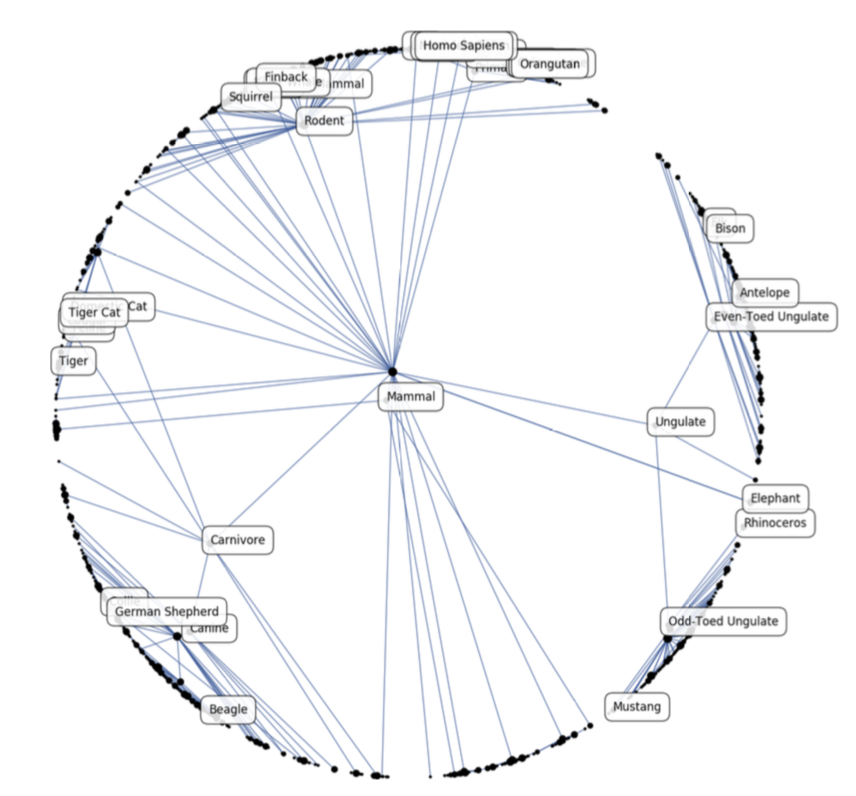
\includegraphics[width=.7\textwidth]{chapter_14/files/poincare-embedding.png}
    \caption{Caption}
    \label{poincare-embedding}
\end{figure}
The measures of efficacy for embeddings of taxonomies are 1) reconstruction of words from embeddings (measured in Mean Average Precision of the ranking of all nouns) 2) link predictions by randomly holding out links.
\subsubsection{Network Embeddings}
This is also a task of link prediction in networks but in social networks datasets.  The probability of an edge is modelsed as Fermi-Dirac distribution:
$$P((u,v) = 1 | \Phi)= \frac{1}{e^{(d(u,v)-r)/t}+1}$$
Here, r corresponds to the radius around each point u such that points within this radius are likely to have an edge with u. The parameter t specifies the steepness of the logistic function and influences both average clustering as well as the degree distribution. It can be seen that Poincar\'e embeddings perform again very well on these datasets and – especially in the low-dimensional regime – outperform Euclidean embeddings.
\subsection{Conclusion}
In this paper, they introduced Poincare embeddings for learning representations of symbolic data and showed that they can learn similarity and hierarchy of objects. They introduced a highly parallelizable algorithm for learning that was based on Riemannian optimization. Finally this setup was evaluated on two tasks: learning taxonomies of embeddings of words and link prediction in social network graphs. Poincare embeddings showed promise in both settings. 

  \section{Introduction}
Delaunay graphs have quite useful properties and are well studied. Therefore finding an embedding of a graph such that the resulting set's Delaunay graph is the same as the original graph would allow us to use these properties and the results from the related literature. This paper focuses on embedding trees into the hyperbolic plane with low distortion and with this property, that the Delaunay graph of the embedded points gives the original tree back.
\section{Preliminaries}
\subsection{Delaunay Graphs}
Let's start by some equivalent definitions of the Delaunay graphs.
\begin{definition}
A Delaunay triangulation of a set of points S is a triangulation such that no point of S is inside the circumcircle of any of the triangles of the triangulation. The graph of a Delaunay triangulation is called a Delaunay graph.
\end{definition}

Although this is the usual definition, the paper provides an equivalent one that is more useful for our purposes:

\begin{definition}
A set of vertices in the hyperbolic plane is called a Delaunay graph if vertex pairs are connected if and only if their Voronoi cells intersect.
\end{definition}

\subsection{Cones in the Hyperbolic Plane}
An important tool in the construction will be so-called cones in the hyperbolic plane.

\begin{definition}
Two parallel lines are called limiting parallel or critically parallel if they never \textit{touch} but they get arbitrarily close asymptotically.
\end{definition}

As a simplification, to have an image, think of $y = \frac{1}{x}$ and $y = -\frac{1}{x}$ in the Euclidean plane.

\begin{definition}
Two parallel lines are called divergent parallel or ultraparallel if they have a closest point and they diverge from each other.
\end{definition}

Again, to have a picture in your mind, think of an hyperbola (whose center axis is parallel to x-axis) and its mirror image w.r.t y-axis in the usual Euclidean plane.

It's a simple property that for any point and a line not passing through it, there is some point on the line such that the \textit{segment} from that to the other point is perpendicular to the line. (This part is also true for Euclidean space). Yet another simple yet crucial property is that we can draw a pair of diverging parallel lines from that outside point such that:

\begin{itemize}
    \item They have symmetric angles with the segment
    \item They are limiting parallel the original line in both directions
\end{itemize}

Figure \ref{fig:cone} shows all of these in action. The region bounded by the original line and the constructed limiting line pair is called a \textit{closed cone}. Note that the position of the original line and the outside point, or equivalently the outside point and the symmetric angles determine cone uniquely. We can create arbitrarily (but finitely) many cones whose apex is the same fixed point by taking different rays, which induce different segments, and we can make all these cones disjoint by picking the rays so that the symmetric angles are small enough.

\begin{figure}
    \centering
    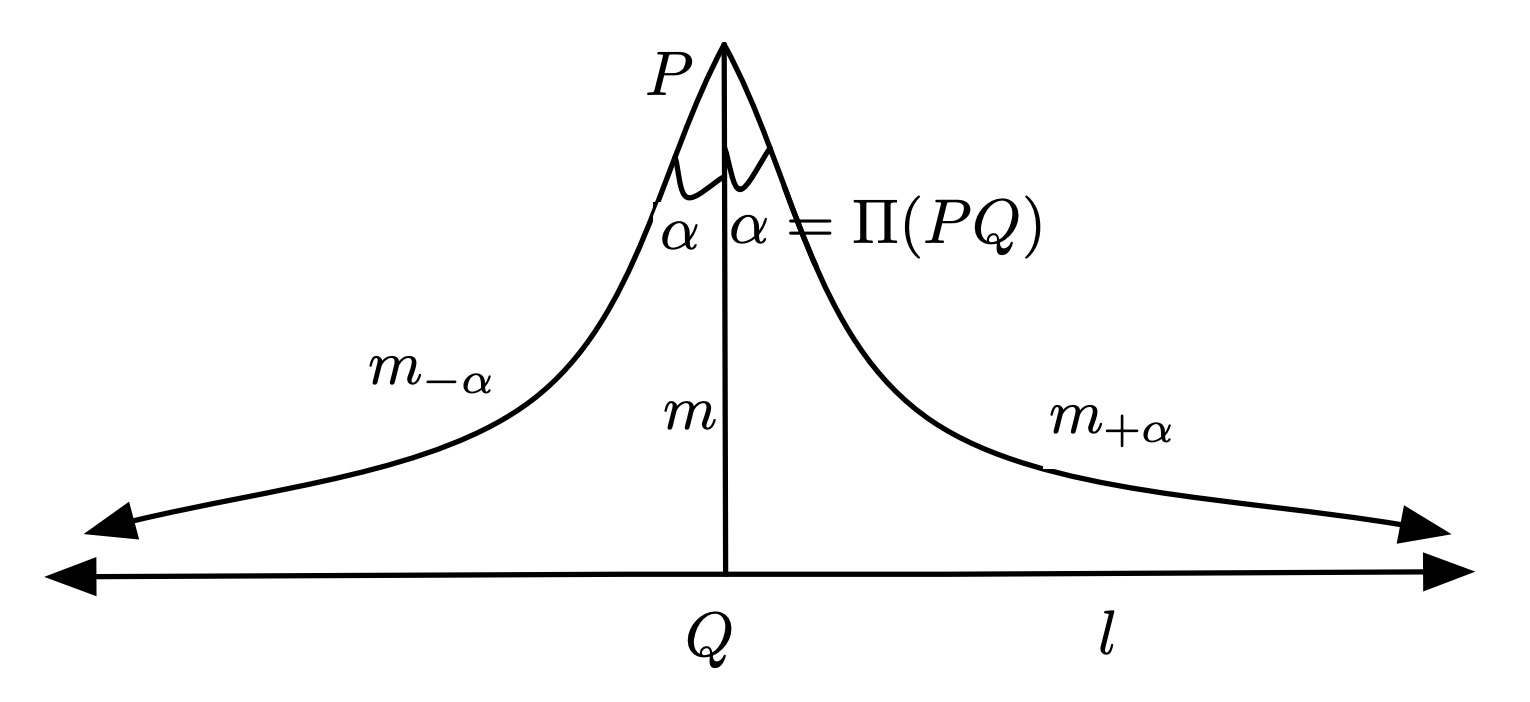
\includegraphics[width=.7\textwidth]{cone.png}
    \caption{Closed Cone}
    \label{fig:cone}
\end{figure}

\section{Delaunay Embeddings of Trees}
First, we will construct an algorithm to embed unweighted trees as Delaunay graphs. We will then gradually build on this embed metric trees \footnote{Weighted tree with shortest path metric} as Delaunay graphs with low distortion.

Consider any vertex as the root to make the tree into a rooted tree. The algorithm is as follows: \\
\horrule{0.5pt} \\
1. Map the root $v_0$ to any point, say $p_0$. \\
2. Delaunay-embed $d$ children of the root into $d$ disjoint cones whose apex are at $p_0$. \\
3. Continue embedding recursively as follows: if $v_i$ is a child of $v_j$, embed children of $v_i$ in disjoint cones that are also disjoint from the $v_i$ $v_j$ embedding cone.  \\
\horrule{0.5pt} \\

\begin{figure}
    \centering
    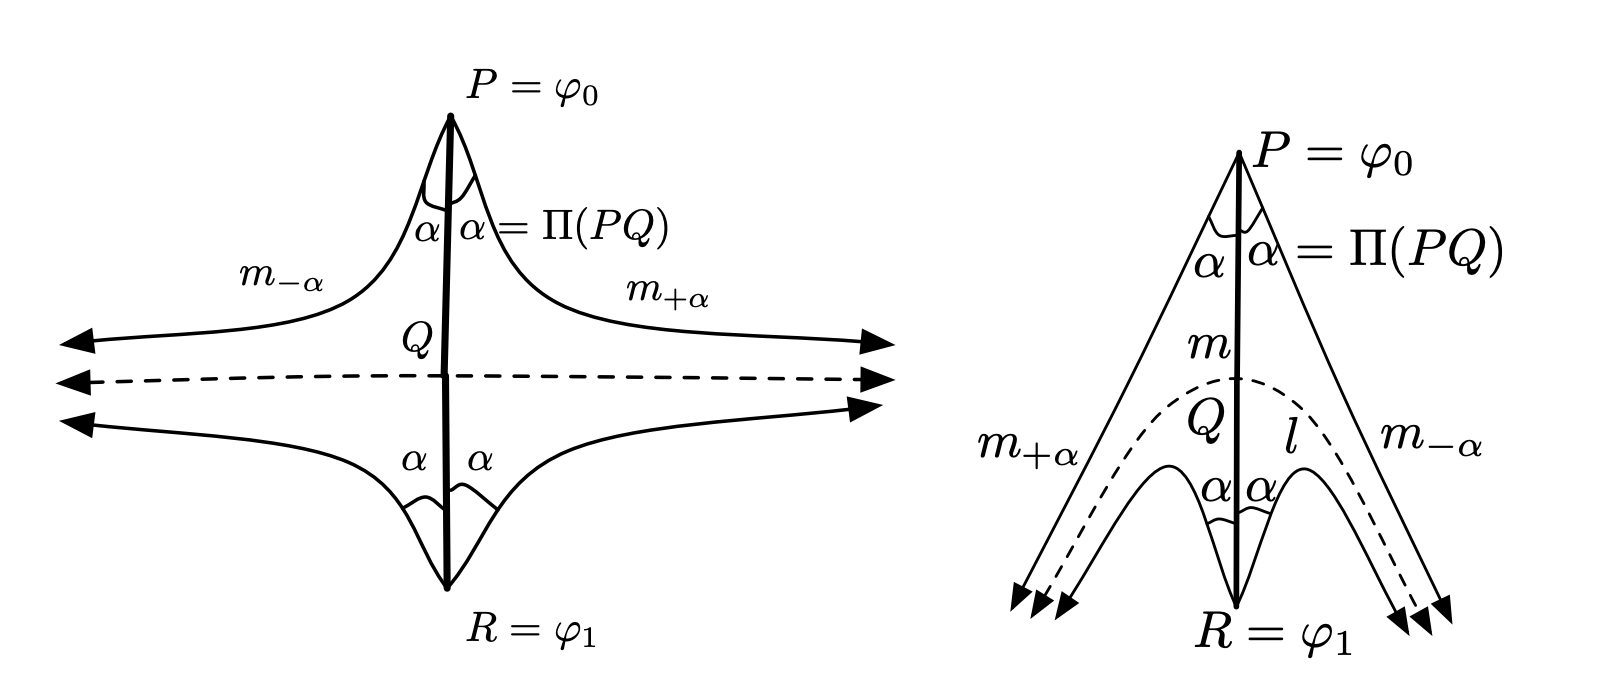
\includegraphics[width=\textwidth]{cone2.png}
    \caption{Embedding of a vertex (at P) and its child (at R), representations from the \textit{points of views} of child and parent respectively}
    \label{fig:cone_two}
\end{figure}

\begin{figure}
    \centering
    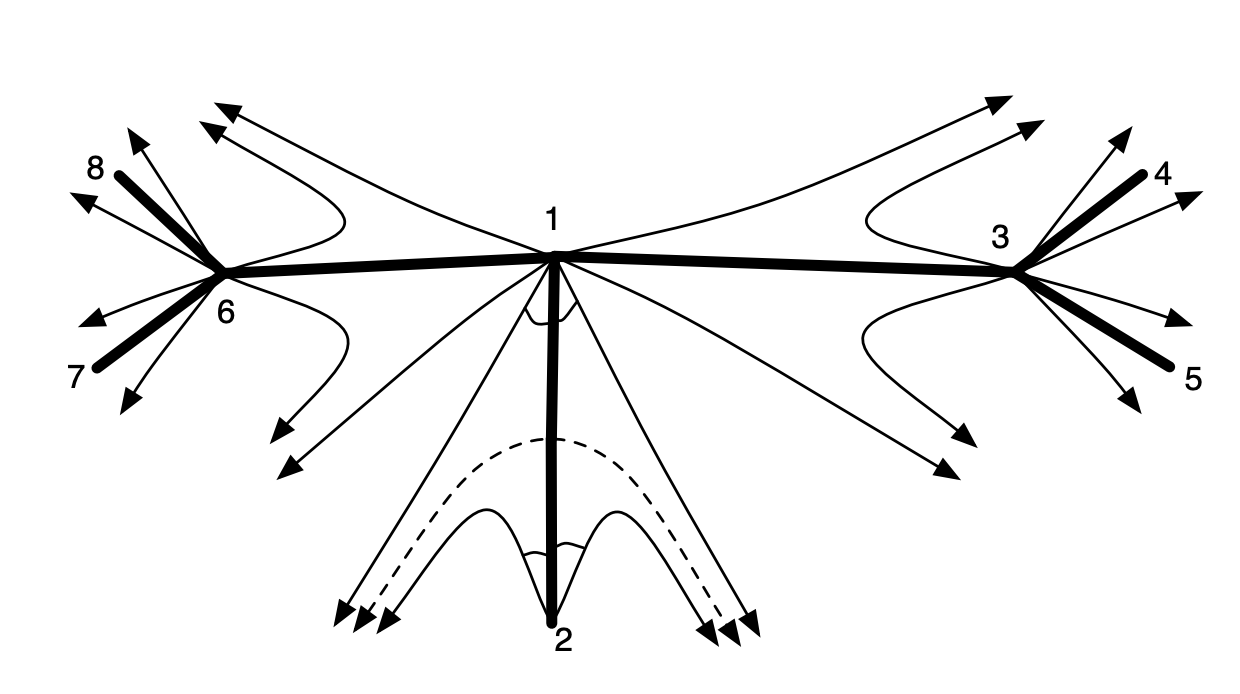
\includegraphics[width=\textwidth]{conem.png}
    \caption{Cone-based representation of the embedding of a whole tree}
    \label{fig:cone_multiple}
\end{figure}

Notice that we assumed we can \textit{Delaunay-embed} individual edges. Here is how we can do it. We choose angles $\alpha$ small enough to ensure disjointness, and for a given edge (one vertex already fixed, say as $p_0$) and its $\alpha$, pick a $p_1$ such that $$|p_0p_1|_{\mathbb{H}} \geq -2k\ln(tan(\frac{\alpha}{2}))$$ See Figures \ref{fig:cone_two} and \ref{fig:cone_multiple} for a visualization.

\section{Delaunay Embeddings of Metric Trees}
Based on the previous embedding, we can actually obtain a stronger one. This time we are considering weighted trees. We want the resulting embedding to capture the \textit{geometry} of the tree, that is, we want the distances of the embedded points to be the same as the weight of the corresponding edge in the original tree (up to a constant that is the same for all edges). We can in fact achieve this, but note that this not the same as embedding a metric tree isometrically: the shortest path distances between vertices that are not adjacent will not stay the same after the embedding. We will denote edge weight between $u$ and $v$ as $w_{u,v}$

The embedding algorithm is quite similar to the unweighted case, and is as follows. For each edge $v_0, v_1$ where $v_0$ is the direct parent of $v_1$,: \\
\horrule{0.5pt} \\
1. Create $degree(v_1) - 1$ cones (whose apex are at embedding of $v_1$) that are disjoint from the $v_0v_1$ embedding cone and also pairwise disjoint (by picking small enough angles). \\
2. Embed children of $v_1$ as follows: Any child $v_2$ is embedded with a cone as before such that $v_1$, $v_2$ distance in the hyperbolic plane is $\eta \cdot w_{v_1, v_2}$  \\
\horrule{0.5pt} \\

Observe that this is the same as the algorithm before, except that we specify the embedding distance more carefully. But again, we embed a child-parent pair as in Figure \ref{fig:cone_two}.

Lastly, we made use of a constant $\eta$. This is a constant which is picked as the maximum of required scaling factors over all edges in the tree. That is, for each edge, there is a minimum scaled factor needed so that the embedded edge is a Delaunay edge. We calculate this number for all edges, and take the maximum over all edges and apply the same scale to all edges so that: (i) all edges are embedded as Delaunay edges, (ii) all edges are scaled by the same amount.

\section{Reducing the Distortion}
As we mentioned above, the embedding we have so far can only guarantee that each edge length will scale by the same factor. However, the distance between vertices that are not adjacent will not scale the same way, since the tree metric can only follow the edges whereas the hyperbolic plane metric is not bound by the edges.

However, it turns out that we can use a similar algorithm that can give an embedding with $1 + \epsilon$ distortion for any $\epsilon > 0$. Note that this involves a trade-off, and see the next section for more details.

\begin{definition}
Two cones that share an apex are $\beta$-separated if they're $2\beta$ angles apart.
\end{definition}

Now, the main theorem that helps us build an embedding with arbitrarily low distortion.

\begin{theorem}
If the following are all true an embedding of a tree, then its distortion is bounded by $1 + \epsilon$
\begin{itemize}
    \item is Delaunay,
    \item all cone pairs used by the embedding are $\beta$-separated for some suitably small constant $\beta$,
    \item all edges are scaled by the same factor $\tau > \eta$ such that each edge becomes longer than $\nu\frac{1+\epsilon}{\epsilon}$, where $\nu$ is a constant that only depends on $\beta$.
\end{itemize}
\end{theorem}

Using this theorem, the following algorithm gives the desired embedding: \\
\horrule{0.5pt} \\
1. Compute the constant $\nu$ and the cone angle $\alpha$ as follows: Find small enough $\beta$ ($< \frac{\pi}{d_{max}}$, where $d_{max}$ is the highest degree in tree), then $\nu = -2k\ln(\tan(\frac{\beta}{2}))$ and $\alpha = \frac{2\pi}{d_{max}} - 2\beta$.
2. Compute $\eta$ as before. \\
3. Compute $\tau$ such that all edges become longer than $\nu\frac{1+\epsilon}{\epsilon}$.
4. Use the embedding algorithm from the previous section, but scale by  $\tau$ instead of $\eta$ and enforce $\beta$-separated cones.\\
\horrule{0.5pt} \\
  % contributors: Cynthia Gao
\section{Representation Trade-Offs for Hyperbolic Embeddings}
Now we will look at \cite{tradeoff}. This paper builds on the previous studies of hyperbolic embedding. 
\cite{Sarkar} has presented an embedding of trees into a Poincar\'e disk. In \cite{tradeoff} the authors analyze the construction by Sarkar and examine the fundamental trade-off between precision and dimensionality. They propose a hyperbolic generalization of multidimentional scaling (h-MDS) for general metric spaces and show that exact recovery of hyperbolic points from distances can be found with the help of perturbation analysis. In stead of using traditional PCA, the authors provide new results for convergence for Principal Geodesic Analysis (PGA).  An SGD-based algorithm, which is initialized with a h-MDS solution, is implemented to recover the submanifold the data is on with losses derived from PGA loss. 


\subsection{Background}
\subsubsection{Hyperbolic spaces}

An important example of hyperbolic space is the Poincar\'e disk $\mathbb{H}_2$ and its generalization $\mathbb{H}_r$ in higher dimensions. Mapping between hyperbolic and Euclidean space preserves angles but not distances, which are given by
\begin{align*}
    d_H(x, y) = \text{acosh}(1 + 2 \frac{||x-y||^2}{(1-||x||^2)(1 - ||y||^2)}),
\end{align*}
where $d_H(x, y)$ represents the hyperbolic distance between two points $x, y$. One property that arises from this mapping is that the shortest path between two points is almost the same as the path through the origin. For the points $||x||=||y|| = t$ with origin $0$, the ratio $\frac{d_E(x, y)}{d_E(x, 0) + d_E(0, y)}$ is constant with respect to $t$ in Euclidean space, whereas $\frac{d_H(x, y)}{d_H(x, 0) + d_H(0, y)}$ approaches 1. In other words, hyperbolic space has a tree-like property which holds far arbitrarily small angles between $x$ and $y$: the shortest path between two neighboring nodes is the path that goes through ther parent (the origin). Another important geometric fact used in the algorithm is that isometric reflection across geodesics can be represented as circle inversion in Euclidean model. 

\subsubsection{Embedding}
Some fidelity measures for embeddings are presented below. One local metric is mean average precision (MAP). For a graph $G = (V, E)$, $a \in V$ has neighborhood $N_a = \{b_1, b_2, \cdots, b_{\deg(a)}\}$. For an embedding $f$, we define $R_{a, b_i}$ to be the smallest set of points that contains $b_i$ that are closest to $f(a)$. MAP is defined to be 
\begin{align*}
    MAP(f) = \frac{1}{|V|} \sum_{a\in V}\frac{1}{\deg(a)} \sum^{|N_a|}_{i=1}\frac{|N_a \cap R_{a, b_i}|}{|R_{a, b_i}|}.
\end{align*}
As a local measure, MAP describes how well the mapping preserves each vertex's neighborhood. $MAP(f) \leq 1$ and equality holds when all neighborhoods are preserved. 

Another important metric used is distortion $D$. For $f:U\rightarrow V$ for $U, V$ with distances $d_U, d_V$ respectively, the distortion is defined as
\begin{align*}
    D(f) = \frac{1}{\binom{n}{2}}\left(\sum_{u, v \in U, u != v}\frac{|d_V(f(u), f(v)) - d_U(u, v)|}{d_U(u, v)}\right)
\end{align*}
When $D(f) = 0$, there is no distortion of edge lengths due to the embedding. $D$ is a global metric because it depends on the related distances rather than local structures. A related metric, the worst case distortion $D_{wc}$ is defined by
\begin{align*}
    D_{wc}(f) = \frac{\max d_V(f(u), f(v))/d_U(u, v)}{\min d_V(f(u), f(v))/d_U(u, v)}.
\end{align*}


\subsection{Hyperbolic Tree Embedding}
Sarkar has shown that it is possible to embed trees into a Poincar\'e disk $\mathbb{H}_2$ with arbitrarily low distortion, which motivates the process for embedding hierarchies into hyperbolic space: 1. First, we embed the graph $G = (V, E)$ into a tree $T$. 2. Then, we embed $T$ into the Poincar\'e ball $\mathbb{H}_d$. This process is referred to as the combinatorial construction. The second step is accomplished by Sarkar's construction. 

Suppose a node $a$ and its parent $b$ are already embedded into $\mathbb{H}_2$, Sarkar's algorithm places the children of $a$ into the hyperbolic disk. $f(a), f(b)$ are reflected across a geodesic so that $f(a)$ is mapped onto the origin and $f(b)$ to some point z. Then the children are placed around a circle with radius $\frac{e^\tau - 1}{e^\tau + 1}$ for some scaling factor $\tau$. They are maximally separated from the reflected node $z$. After reflecting every points back across the geodesic, the isometric properties of hyperbolic space guarantees that all the children are $d_H = \tau$ away from $f(a)$. 

\subsubsection{Analysis of Sarkar's Construction}

Sarkar's construction produces a Delauney embedding, which is able to preserve the neighborhoods - nodes that are in the same cluster will be mapped to the same area. However, hyperbolic space is not scale invariant. The increase in scale preserves the distance between nodes that are farther apart better, hence the trade-off: if we want a better distortion, we have to pay for it in precision, the largest norm of a point determined by the longest path in the tree. It turns out that the precision is logarithmically proportional to the degree of the tree but linearly proportional to the maximum path length. In other words, hyperolic embeddings with short trees with more branches requires less bits of precision and longer trees gives less distortion but worse precision.  

With $b$ bits of precision, we can represent $2^b$ distinct points, so the bit complexity for $\epsilon$-covered ball $B(0, d)$ is of $n\log(d/\epsilon)$ in a Euclidean space and $O(d)$ in hyperbolic space. If $x \in \mathbb{H}_2, ||x|| < 1$, we need enough bits so that $1 - ||x||$ will not be rounded to zero, which requires about $ -\log(1 - ||x||)$ bits. For two points $x, y$ and their reflection across geodesic $(0, z)$, we have 
\begin{align*}
    d = d_H(x, y) = d_H(0, z) = \text{acosh}(1 + 2 \frac{||z||^2}{1 - ||z||^2})\\
    \frac{\cosh{d}+1}{2} \geq \frac{1/2}{1 - ||z||}.
\end{align*}
The number of bits we need is $\log(\cosh(d)+1)$, which is roughly $d$ bits. Therefore, we needs $d$ bits in hyperbolic space rather than $\log d$ in Euclidean space. 

Denote the longest path in the tree by $l$. If we have $\tau = \frac{1}{\epsilon}(2 \log \frac{\deg_{\max}}{\pi/2})$, the largest distance is $O(\frac{l}{\epsilon} \log \deg_{\max})$ and number of bits for representation is on the same order. This expression explains why a short, bushy tree is not penalized as much in precision as a taller tree. By selecting a graph with $m(\deg_{\max} + 1)$ nodes in a tree that has $\deg_{\max}$ chains of length $m$, we can prove that the lower bound is $\Omega(\frac{l}{\epsilon} \log \deg_{\max})$.

Sarkar's algorithm can be generalized to a higher dimension with ball $\mathbb{H}_r$. Instead of placing the children on a disk, we put them at the vertices of a hypercube inscribed into the unit hypersphere. The points can be represented by
\begin{align*}
    x_a = \left(\frac{(-1)^{a_1}}{\sqrt{r}}, \cdots, \frac{(-1)^{a_r}}{\sqrt{r}}\right),
\end{align*}
where $a \in \{0, 1\}^r$. The scaling factor can be reduced by increasing the dimension, because we can place more children with larger angles between them. Thus, for a higher dimension and $\mathbb{H}_r$, we require at most $O(\frac{l}{\epsilon} \frac{l}{r} \log \deg_{\max})$ bits for representation for $r \leq (\log \deg_{\max}) + 1$, and $O(\frac{1}{\epsilon}l)$ bits for $r > (\log \deg_{\max}) + 1$.  

As for the first step, embedding graphs into trees, there are some limitations on this transformation. Breaking a cycle would lead to larger distortion in general. Steiner nodes are added to help embed long cycles: connecting a Steiner node to all the rest of the node with proper edge weight recovers the distance between any pair of nodes in the graph with a tree-like property. In conclusion, we have to balance precision and quality for hyperbolic embeddings. For short, bushy trees, hyperbolic embeddings do very well, whereas for trees with long paths, they do less well because the order of bits is directly proportional to the path length. 

\subsection{Hyperbolic Multidimensional Scaling}

For a set of hyperbolic points $x_1, \cdots, x_n \in \mathbb{H}_2$, we have the pairwise distance $d_{i, j} = d_H(x_i, x_j)$ and want to recover the points in a matrix form $X \in \mathbb{R}^{n \times r}$. In Euclidean space, the multidimensional scaling assumes all the points have mean zero and recovers a centered embedding. In hyperbolic space, we have to make slight modifications, including a pseudo-Euclidean mean that enables matrix factorization. We use a hyperboloid model, which can be easily converted to the Poincar\'e ball. The problem can be converted to a standard PCA and the centering helps to preserve submanifolds as well.

Let $Q \in \mathbb{R}^{r+1}$ be the diagonal matrix with $Q_{00} = 1, Q_{ii} = -1$. The hyperboloid model is defined as 
\begin{align*}
    \mathbb{M}_r = {x \in \mathbb{R}^{r+1}|x^TQx = 1 \wedge x_0 > 0},
\end{align*}
with its distance measure
\begin{align*}
    d_H(x, y) = \text{acosh}(x^TQy).
\end{align*}
As for the new mean, we define a variance term in hyperbolic space
\begin{align*}
    \Psi(z; x_1, \cdots, x_n) = \sum^n_{i=1}\sinh^2(d_H(x_i, z)).
\end{align*}
Our pseudo-Euclidean mean is the local minimum of the above $\Psi$. For matrix $X \in \mathbb{R}^{n \times r}$ such that $X^Te_i = \Vec{x}_i$ and $u \in \mathbb{R}^n$ such that $u_i = x_{0, i}$, we take the gradient of the variance term and get
\begin{align*}
    \nabla_z \Psi(z; x_1, \cdots, x_n)|_{z= 0} = -2 \sum^n_i x_{0, i}\Vec{x}_i = -2X^Tu. 
\end{align*}
In this way, the hyperbolic points are centered if $X^Tu = 0$. 

Suppose we have $x_1, \cdots, x_n$ and their pairwise distances $d_H(x_i, x_j)$, we can compute the matrix $Y$ such that 
\begin{align*}
    Y_{i, j} = \cosh(d_H(x_i, x_j)) = x_i^TQx_j = x_{0, i}x_{0, j} - \Vec{x}_i^T\Vec{x}_j = uu^T - XX^T.
\end{align*}
Assuming the points are centered, $X^Tu = 0$, $u$ becomes an eigenvector of $Y$. It turns out that running PCA on $-Y = X^TX - uu^T$ and compute $n$ most significant non-negative eigenvectors recovers $X$ up to rotation. Then we can find $u$ from $x_0 = \sqrt{1 + ||\Vec{x}||^2}$. Therefore, the algorithm for h-MDS proposed with input distance matrix $d_{i, j}$ and rank $r$ is \\
\rule{\linewidth}{0.5pt} \\
1. Compute scaled distance $Y_{i, j} = \cosh(d_{i, j})$\\
2. Compute $X$ from performing PCA on $(-Y, r)$\\
3. Project $X$ from hyperboloid model to Poincar\'e model: $x \rightarrow \frac{x}{1 + \sqrt{1 + ||x||^2}}$\\
4. Center $X$ to a different mean if needed. \\
\rule{\linewidth}{0.5pt} \\

\subsubsection{PGA}
If we want to perform dimensionality reduction to the high-rank embedding in hyperbolic space, we follow Principal Geodesic Analysis (PGA). Our goal is to find a geodesic $\gamma: [0, 1] \rightarrow \mathbb{H}_2$ that passes through mean of the points and minimizes the squared error:
\begin{align*}
    f(\gamma) = \sum^n_{i=1} \min_t d_H(\gamma(t), x_i)^2. 
\end{align*}
In a Poincar\'e model, the reflection across a geodesic that passes through the origin is the same in both Euclidean and hyperbolic space. For a line through origin $\gamma$ and its reflection $R_\gamma$, we have
\begin{align*}
    d_H(\gamma, x) = \min_t d_H(\gamma(t), x) = \frac{1}{2}d_H(R_l x, x).
\end{align*}
Using the hyperbolic metric, we get 
\begin{align*}
    f(\gamma) &= \frac{1}{4}\sum^n_i \text{acosh}^2(1 + \frac{8d_E(\gamma, x_i)^2}{(1 - ||x_i||^2)^2})\\
    &= \frac{1}{4}\sum^n_i \text{acosh}^2(1 + d_E(\gamma, w_i)^2),
\end{align*}
where $w_i = \sqrt{8}x_i/(1 - ||x_i||^2)$ for simplification. 

However, unlike PCA, the loss function is not convex, which means there could be multiple local minima. It is still possible to give a sufficient condition on the data so that $f$ becomes convex: if for all $i$, we have 
\begin{align*}
    \text{acosh}^2(1 + d_E(\gamma, w_i)^2) < \min(1, \frac{1}{3}||w_i||^2),
\end{align*}
then $f$ is locally convex at $\gamma$. 


  \printbibliography[heading=subbibliography]
\end{refsection}














% \end{document}


